\documentclass[]{auvsi_doc}
\setkeys{auvsi_doc.cls}{
	AUVSITitle={Airframe Subsystem Description},
	AUVSILogoPath={./../logo.pdf}
}

% include extra packages, if needed

\begin{document}

\begin{AUVSITitlePage}
\begin{artifacttable}
\entry{AF??, 0.1, 02-14-19, Initial Draft, Tyler Critchfield, CHECKED BY}
% additional \entry{} commands for extra rows in the revision table, if needed
\end{artifacttable}
\end{AUVSITitlePage}

% document contents (see below for LaTex commands that make your life easier)
\section{Introduction}
This artifact describes the final design of the Nimbus Pro airframe that was the chosen design concept in the Concept Development stage. Images of the built airframe are included, as well as a list of modifications we made to the plane. We then describe how this concept helps us achieve our key success measures.

\section{Design Description}
Our airframe is the Nimbus Pro aircraft we selected as our chosen design in the Concept Development stage. It is a fixed-wing plane with a large storage capacity and large wing span made of polystyrene (Fig \ref{fig:plane1}).

\begin{figure}[h!]
	\centering
	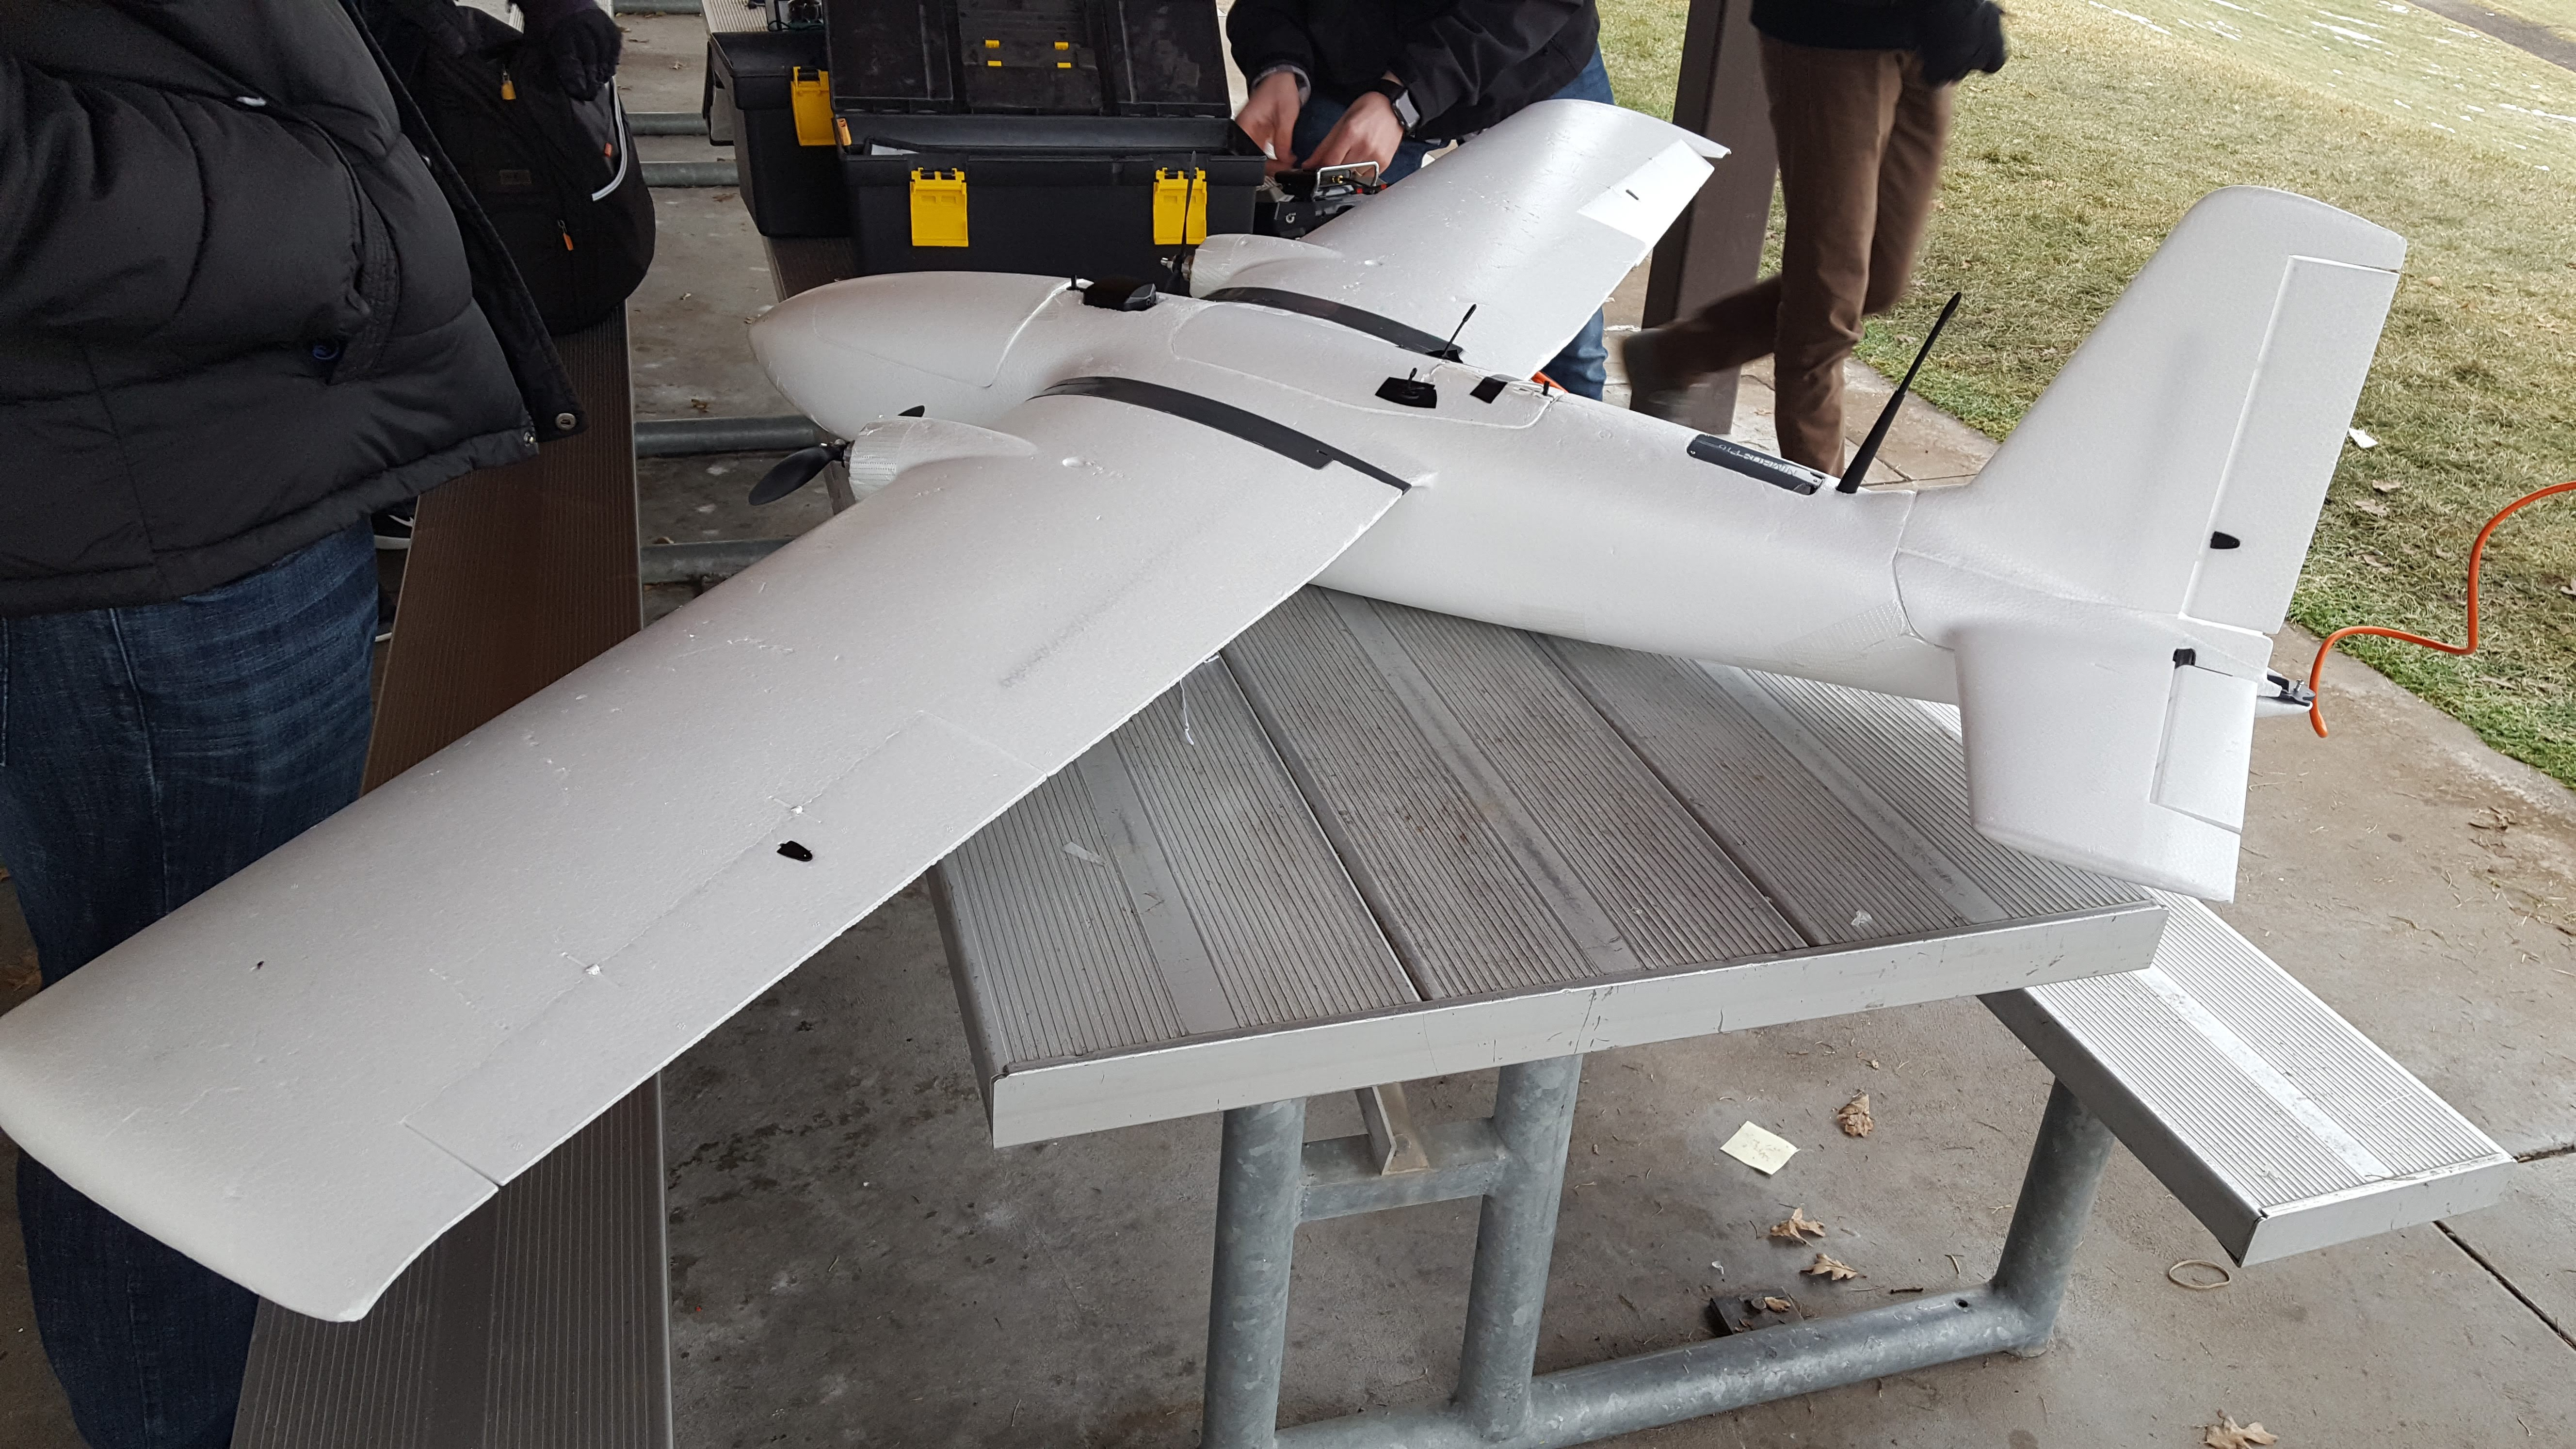
\includegraphics[width=.9\columnwidth]{plane1}
	\caption{Fully-constructed Nimbus Pro airframe before its first flight.}
	\label{fig:plane1}
\end{figure} 




\end{document}
